%Este trabalho está licenciado sob a Licença Atribuição-CompartilhaIgual 4.0 Internacional Creative Commons. Para visualizar uma cópia desta licença, visite http://creativecommons.org/licenses/by-sa/4.0/deed.pt_BR ou mande uma carta para Creative Commons, PO Box 1866, Mountain View, CA 94042, USA.

\documentclass[12pt]{article}

\input ../preambulo.tex
\input ../preambulo_python.tex

\lstset{
%  belowcaptionskip = 0em,
  belowskip = 0em
}
\makeindex

\begin{document}

\title{Python para Matemática}
\author{Pedro H A Konzen}
\date{\today}

\maketitle

\tableofcontents

\section{Licença}\label{sec_licenca}

Este trabalho está licenciado sob a Licença Atribuição-CompartilhaIgual 4.0 Internacional Creative Commons. Para visualizar uma cópia desta licença, visite http://creativecommons.org/licenses/by-sa/4.0/deed.pt\_BR ou mande uma carta para Creative Commons, PO Box 1866, Mountain View, CA 94042, USA.


\section{Sobre a Linguagem}\label{sec_sobrepy}

\hl{{\python} é uma \emph{linguagem de programação} de \emph{alto nível} e \emph{multiparadigma}}. Ou seja, é relativamente próxima das linguagens humanas naturais, é desenvolvida para aplicações diversas e permite a utilização de diferentes paradigmas de programação (programação estruturada, orientada a objetos, orientada a eventos, paralelização, etc.).

\begin{itemize}
\item \hlemph{Site oficial}
  \begin{center}
    \href{https://www.python.org/}{https://www.python.org/}
  \end{center}
\end{itemize}

\subsection{Instalação e Execução}

\hl{Para executar um código {\python} em seu computador é necessário instalar um \emph{interpretador}}. No \href{https://www.python.org/}{site oficial}, estão disponíveis para \textit{download} interpretadores gratuitos e com licença livre para uso. Neste minicurso, vamos utilizar \emph{Python 3}.

\subsubsection{Online Notebook}

\hl{Usar um \emph{\textit{Notebook} {\python} \textit{online}} é uma forma rápida e prática de iniciar os estudos na linguagem}. Rodam diretamente em nuvem e vários permitem o uso gratuito por tempo limitado. Algumas opções são:
\begin{itemize}
\item \href{https://deepnote.com}{Deepnote} - \url{https://deepnote.com}
\item \href{https://colab.research.google.com/}{Google Colab} - \url{https://colab.research.google.com/}
\item \href{https://www.kaggle.com/}{Kaggle} - \url{https://www.kaggle.com/}
\item \href{https://www.paperspace.com/notebooks}{Paperspace Gradient} - \url{https://www.paperspace.com/notebooks}
\item \href{https://aws.amazon.com/sagemaker/}{SageMaker} - \url{https://aws.amazon.com/sagemaker}
\end{itemize}

\subsubsection{IDE}

\hl{Usar um \emph{ambiente integrado de desenvolvimento} (IDE, em inglês, \textit{integrated development environment}) é a melhor forma de capturar o todo o potencial da linguagem {\python}}. Algumas alternativas são:
\begin{itemize}
\item \href{https://docs.python.org/3/library/idle.html}{IDLE} - \url{https://docs.python.org/3/library/idle.html}
\item \href{https://www.gnu.org/software/emacs/download.html}{GNU Emacs} - \url{https://www.gnu.org/software/emacs/}
\item \href{https://www.spyder-ide.org/}{Spyder} - \url{https://www.spyder-ide.org/}
\item \href{https://code.visualstudio.com/}{VS Code} - \url{https://code.visualstudio.com/}
\end{itemize}

\subsection{Utilização}

A \hl{execução de códigos {\python}} pode ser feita de três formas básicas:
\begin{itemize}
\item \hl{em modo interativo em um console/\textit{notebook} {\python}};
\item \hl{por execução de um código \texttt{arqnome.py} em um console/\textit{notebook} {\python}};
\item \hl{por execução de um cógido \texttt{arqnome.py} em um terminal do sistema operacional}.
\end{itemize}

\begin{ex}
  Consideramos o seguinte pseudocódigo.

\begin{verbatim}
s = "Ola, mundo!".
imprime(s). (imprime a string s)
\end{verbatim}

Vamos escrevê-lo em {\python} e executá-lo:

\begin{enumerate}[a)]
  \item Em um \textit{notebook}.
  
  Iniciamos um \textit{notebook} {\python} e digitamos o seguinte código em uma célula de entrada.

\begin{lstlisting}
s = "Olá, Mundo!"
#imprime a string s
print(s)
\end{lstlisting}

  Ao executarmos a célula, obtemos a saída

\begin{verbatim}
Olá, Mundo!
\end{verbatim}

  \item Em modo iterativo no console.
  
  Iniciamos um console {\python} em terminal do sistema e digitamos

\begin{verbatim}
$ python3
\end{verbatim}

Aqui, \texttt{\$} é o símbolo de \textit{prompt} de entrada que pode ser diferente a depender do seu sistema operacional. Então, digitamos

\begin{lstlisting}
>>> s = "Olá, Mundo!"
>>> print(s) #imprime a string s
\end{lstlisting}

Observamos que \lstinline+>>>+ é o símbolo de \textit{prompt} de entrada do console {\python}. A saída 

\begin{lstlisting}
Olá, Mundo!
\end{lstlisting}

aparece logo abaixo da última linha de \textit{prompt} executada. Para encerrar o console, digitamos

\begin{lstlisting}
>>> quit()
\end{lstlisting}
  
  \item Escrevendo o código \verb+ola.py+ e executando-o em um console/\textit{notebook} {\python}.
  
  Primeiramente, escrevemos o código

\begin{lstlisting}
s = "Olá, Mundo!"
print(s) # imprime a string s
\end{lstlisting}

em um IDE (ou em um simples editor de texto) e salvamo-lo no caminho \texttt{/caminho/ola.py}. Então, o executamos no console/\textit{notebook} {\python} com

\begin{lstlisting}
exec(open('/pasta/codigo.py').read())
\end{lstlisting}

A saída é impressa logo abaixo do \textit{prompt}/célula de entrada.
  
  \item Escrevendo o código \verb+ola.py+ e executando-o em terminal do sistema.
  
  Assumindo que o código já esteja salvo no arquivo \texttt{/caminho/ola.py}, podemos executá-lo em um terminal digitando

\begin{lstlisting}
$ python3 /caminho/ola.py
\end{lstlisting}

  A saída é impressa logo abaixo do \textit{prompt} de entrada do sistema.
\end{enumerate}

\end{ex}

\section{Elementos da Linguagem}\label{sec_elem}

\subsection{Classes de Objetos Básicos}

\hl{{\python} é uma \emph{linguagem} de programação \emph{dinâmica} em que as variáveis/objetos são declaradas/os automaticamente ao receberem um valor/dado}. Por exemplo, consideramos as seguintes instruções

\begin{lstlisting}
x = 2
y = x * 3.0
\end{lstlisting}

Na primeira instrução, a variável \texttt{x} recebe o valor inteiro \texttt{2} e, então, é armazenado na memória do computador como um objeto da \hl{classe {\PYTHONint}} (número inteiro). Na segunda instrução, \texttt{y} recebe o valor decimal $6.0$ (resultado de $2\times 3.0$) e é armazenado como um objeto da \hl{classe {\PYTHONfloat}} (ponto flutuante de 64-{\it bits}). Podemos verificar isso, com as seguintes instruções

\begin{lstlisting}
print(x)
\end{lstlisting}

\begin{verbatim}
  2
\end{verbatim}

\begin{lstlisting}
print(y)
\end{lstlisting}

\begin{verbatim}
  6.0
\end{verbatim}

\begin{lstlisting}
print(type(x), type(y))
\end{lstlisting}

\begin{verbatim}
  <class 'int'> <class 'float'>
\end{verbatim}

\begin{obs}\normalfont{(\hl{Comentários e Continuação de Linha}.)}
  Códigos {\python} admitem \emph{comentários} e \emph{continuação de linha} como no seguinte exemplo

\begin{lstlisting}
# isto é um comentário
s = "isto é uma \
string"
print(s)
\end{lstlisting}

\begin{verbatim}
  isto é uma string
\end{verbatim}

\begin{lstlisting}
  type(s)
\end{lstlisting}

\begin{verbatim}
  <class 'str'>
\end{verbatim}

\end{obs}

\begin{obs}\normalfont{(\hl{Notação científica}.)}
  O {\python} aceita \emph{notação científica}. Por exemplo $5.2\times 10^{-2}$ é digitado da seguinte forma

\begin{lstlisting}
5.2e-2
\end{lstlisting}

\begin{verbatim}
0.052
\end{verbatim}

\end{obs}

\begin{obs}\normalfont{(\hl{\textit{Casting}}.)}
  Quando não há ambiguidade, pode-se fazer a conversão entre objetos de classes diferentes (\textit{casting}). Por exemplo,

\begin{lstlisting}
x = 1
print(x, type(x))
\end{lstlisting}

\begin{verbatim}
  1 <class 'int'>
\end{verbatim}

\begin{lstlisting}
y = float(x)
print(y, type(y))
\end{lstlisting}

\begin{verbatim}
1.0 <class 'float'>  
\end{verbatim}

\end{obs}

Além de objetos numéricos e {\it string}, {\python} também conta com objetos {\PYTHONlist} (lista), {\PYTHONtuple} ($n$-upla) e {\PYTHONdict} (dicionário). Estudaremos essas classes de objetos mais adiante no minicurso.

\begin{exr}
  Antes de implementar, diga qual o valor de \texttt{x} após as seguintes instruções.

\begin{lstlisting}
x = 1
y = x
y = 0
\end{lstlisting}

Justifique seu resposta e verifique-a.
\end{exr}

\begin{exr}
  Implemente um código em que a(o) usuária(o) entra com valores para as variáveis \texttt{x} e \texttt{y}. Então, os valores das variáveis são permutados entre si. Dica: use {\PYTHONinput} para a entrada de dados.
\end{exr}

\subsection{Operações Aritméticas Elementares}

Os operadores aritméticos elementares são:
\begin{itemize}
\item[] \lstinline-+- \hlemph{adição}
\item[] \lstinline+-+ \hlemph{subtração}
\item[] \lstinline+*+ \hlemph{multiplicação}
\item[] \lstinline+/+ \hlemph{divisão}
\item[] \lstinline+**+ \hlemph{potenciação}
\item[] \lstinline+\%+ \hlemph{módulo}
\item[] \lstinline+//+ \hlemph{divisão inteira}
\end{itemize}

\begin{ex}
  Estudamos a seguinte computação

\begin{lstlisting}
2+8*3/2**2-1
\end{lstlisting}

\begin{verbatim}
7.0
\end{verbatim}

Observamos que as operações \lstinline+**+ tem precedência sobre as operações \lstinline+*+, \lstinline+/+, \lstinline+\%+, \lstinline+//+, as quais têm precedência sobre as operações \lstinline!+, -!. Operações de mesma precedência seguem a ordem da esquerda para direita, conforme escritas na linha de comando. Usa-se parênteses para alterar a precedência entre as operações, por exemplo

\begin{lstlisting}
(2+8*3)/2**2-1
\end{lstlisting}

\begin{verbatim}
5.5
\end{verbatim}

\end{ex}

\begin{obs}\normalfont{(\hl{Precedência das Operações}.)}
Consulte mais informações sobre a precedência de operadores em \href{https://docs.python.org/3/reference/expressions.html#operator-precedence}{Python Docs: Operator Precedence}.
\end{obs}

\begin{exr}\label{exr:bhaskara}
  Compute as raízes do seguinte polinômio quadrático
  \begin{equation}
    p(x) = 2x^2 - 2x - 4
  \end{equation}
  usando a fórmula de Bhaskara{\bhaskara}.
\end{exr}

O operador \lstinline+\%+ módulo computa o \emph{resto da divisão} e o operador \lstinline+//+ a \emph{divisão inteira}, por exemplo

\begin{lstlisting}
>>> 5 % 2
\end{lstlisting}

\begin{verbatim}
1
\end{verbatim}

\begin{lstlisting}
5 // 2
\end{lstlisting}

\begin{verbatim}
2
\end{verbatim}

\begin{exr}
  Use o {\python} para computar os inteiros não negativos $q$ e $r$ tais que
  \begin{equation}
    25 = q\cdot 3 + r,
  \end{equation}
  sendo $r$ o menor possível.
\end{exr}

\subsection{Funções e Constantes Elementares}

\hl{O \emph{módulo} Python {\PYTHONmath} disponibiliza várias funções e constantes elementares}. Para usá-las, precisamos importar o módulo em nosso código

\begin{lstlisting}
import math
\end{lstlisting}

Com isso, temos acesso a todas as definições e declarações contidas neste módulo. Por exemplo

\begin{lstlisting}
math.pi
\end{lstlisting}

\begin{verbatim}
3.141592653589793
\end{verbatim}

\begin{lstlisting}
math.cos(math.pi)
\end{lstlisting}

\begin{verbatim}
-1.0
\end{verbatim}

\begin{lstlisting}
math.sqrt(2)
\end{lstlisting}

\begin{verbatim}
1.4142135623730951
\end{verbatim}

\begin{lstlisting}
math.log(math.e)
\end{lstlisting}

\begin{verbatim}
1.0
\end{verbatim}


\begin{obs}\normalfont{(\hl{Função Logaritmo}.)}
  Notamos que {\PYTHONmathDOTlog} é a função logaritmo natural, i.e. $\ln(x) = \log_e(x)$. A implementação {\python} para o logaritmo de base 10 é {\PYTHONmathDOTlog}\texttt{(x, 10)} ou, mais acurado, {\PYTHONmathDOTlogTen}.
\end{obs}

\begin{exr}
  Compute
  \begin{enumerate}[a)]
  \item $\displaystyle \sen\left(\frac{\pi}{4}\right)$
  \item $\displaystyle e^{\log_3(\pi)}$
  \item $\displaystyle \sqrt[3]{-27}$
  \end{enumerate}
\end{exr}

\begin{exr}
  Refaça o Exercício~\ref{exr:bhaskara} usando a função {\PYTHONmathDOTsqrt} para computar a raiz quadrada do discriminante.
\end{exr}

\subsection{Operadores de Comparação Elementares}

Os \hlemph{operadores de comparação} elementares são
\begin{itemize}
\item[]\lstinline+==+ \hlemph{igual a}
\item[]\lstinline+!=+ \hlemph{diferente de}
\item[]\lstinline+>+ \hlemph{maior que}
\item[]\lstinline+<+ \hlemph{menor que}
\item[]\lstinline+>=+ \hlemph{maior ou igual que}
\item[]\lstinline+<=+ \hlemph{menor ou igual que}
\end{itemize}
Estes operadores \hl{retornam os \emph{valores lógicos} {\PYTHONTrue} (verdadeiro) ou {\PYTHONFalse} (falso)}.

Por exemplo, temos

\begin{lstlisting}
x = 2
x + x == 4
\end{lstlisting}

\begin{verbatim}
True
\end{verbatim}

\begin{exr}
  Considere a circunferência de equação
  \begin{equation}
    c: ~(x - 1)^2 + (y + 1)^2 = 1.
  \end{equation}
  Escreva um código em que a(o) usuária(o) entra com as coordenadas de um ponto $P = (x, y)$ e o código verifica se $P$ pertence ao disco determinado por $c$.
\end{exr}

\begin{exr}
  Antes de implementar, diga qual é o valor lógico da instrução

\begin{lstlisting}
math.sqrt(3)**2 == 3
\end{lstlisting}

Justifique sua resposta e verifique!
\end{exr}

\subsection{Operadores Lógicos Elementares}

Os \hlemph{operadores lógicos} elementares são:
\begin{itemize}
\item[]\texttt{and} \hlemph{\texttt{e} lógico}
\item[]\texttt{or} \hlemph{\texttt{ou} lógico}
\item[]\texttt{not} \hlemph{\texttt{não} lógico}
\end{itemize}

\begin{ex}\normalfont{(\hl{Tabela Booleana do \texttt{and}}.)}
  A tabela booleana{\boole} do \texttt{and} é
  \begin{center}
    \begin{tabular}[H]{ll|l}
      \texttt{A} & \texttt{B} & \texttt{A and B}\\\hline
      \texttt{True} & \texttt{True} & \texttt{True} \\
      \texttt{True} & \texttt{False} & \texttt{False} \\
      \texttt{False} & \texttt{True} & \texttt{False} \\
      \texttt{False} & \texttt{False} & \texttt{False} \\\hline
    \end{tabular}
  \end{center}

  Por exemplo, temos

\begin{lstlisting}
x = 2
(x > 1) and (x < 2)
\end{lstlisting}

\begin{verbatim}
False
\end{verbatim}

\end{ex}

\begin{exr}
  Construa as tabelas booleanas do operador \texttt{or} e do \texttt{not}.
\end{exr}

\begin{exr}
  Use {\python} para verificar se $1.4 <= \sqrt{2} < 1.5$.
\end{exr}

\begin{exr}
  Considere um retângulo $r: ~ABDC$ de vértices $A = (1, 1)$ e $D = (2, 3)$. Crie um código em que a(o) usuária(o) informa as coordenadas de um ponto $P = (x, y)$ e o código imprime {\PYTHONTrue} ou {\PYTHONFalse} para cada um dos seguintes itens:
  \begin{enumerate}
  \item $P\in r$.
  \item $P\in \p r$.
  \item $P\not\in \overline{r}$.
  \end{enumerate}
\end{exr}

\begin{exr}
  Implemente uma instrução para computar o operador \texttt{xor} (ou exclusivo). Dadas duas afirmações \texttt{A} e \texttt{B}, \texttt{A xor B} é {\PYTHONTrue} no caso de uma, e somente uma, das afirmações ser {\PYTHONFalse}, caso contrário é {\PYTHONFalse}.
\end{exr}


\subsection{\texttt{set}}

\hl{Um {\PYTHONset} em {\python} é uma \emph{coleção de objetos} \emph{não ordenada}, \emph{imutável} e \emph{não admite itens duplicados}}. Por exemplo,

\begin{lstlisting}
a = {1, 2, 3}
type(a)  
\end{lstlisting}

\begin{verbatim}
  <class 'set'>
\end{verbatim}

\begin{lstlisting}
b = set((2, 1, 3, 3))
print(b)
\end{lstlisting}

\begin{verbatim}
  {1, 2, 3}
\end{verbatim}

\begin{lstlisting}
a == b
\end{lstlisting}

\begin{verbatim}
True
\end{verbatim}

\begin{lstlisting}
# conjunto vazio
e = set()  
\end{lstlisting}

Acima, alocamos o conjunto $a = \{1,2, 3\}$. Note que o conjunto $b$ é igual a $a$. Observamos que o conjunto vazio deve ser construído com a instrução \texttt{set()} e não com \lstinline+{}+\footnote{Isso constrói um dicionário vazio, como estudaremos logo mais.}.

\begin{obs}\normalfont{(\hl{Tamanho de uma Coleção de Objetos}.)}
  A função {\PYTHONlen} retorna o número de elementos de uma coleção de objetos. Por exemplo,
  
\begin{lstlisting}
len(a)
\end{lstlisting}

\begin{verbatim}
3
\end{verbatim}

\end{obs}

\emph{Operadores envolvendo conjuntos}:
\begin{itemize}
\item[] \lstinline+-+ \hl{diferença entre conjuntos}
\item[] \lstinline+|+ \hl{união de conjuntos}
\item[] \lstinline+&+ \hl{interseção de conjuntos}
\item[] \lstinline+^+ \hl{diferença simétrica}
\end{itemize}

\begin{ex}
  Os conjuntos
  \begin{gather}
    A = \{2, \pi, -0.25, 3, \text{'banana'}\},\\
    B = \{\text{'laranja'}, 3, \operatorname{arc cos}(-1), -1\}
  \end{gather}
  podem ser alocados como \texttt{sets}

\begin{lstlisting}
import math
A = {2, math.pi, -0.25, 3, 'banana'}
B = {'laranja', 3, math.acos(-1), -1}
\end{lstlisting}
    
e, então, podemos computar:

  \begin{enumerate}[a)]
  \item $A\setminus B$

\begin{lstlisting}
a = A - B
print(a)
\end{lstlisting}

\begin{verbatim}
{-0.25, 2, 'banana'}
\end{verbatim}

  \item $A\cup B$

\begin{lstlisting}
b =  A | B
print(b)
\end{lstlisting}

\begin{verbatim}
{-0.25, 2, 3, 3.141592653589793, 'laranja', 'banana', -1}
\end{verbatim}
    
  \item $A\cap B$
  
\begin{lstlisting}
c = A & B
print(c)
\end{lstlisting}

\begin{verbatim}
{3, 3.141592653589793}
\end{verbatim}
    

  \item $A\Delta B = (A\setminus B) \cup (B\setminus A)$
  
\begin{lstlisting}
d = A ^ B
print(d)
\end{lstlisting}


\begin{verbatim}
{-0.25, 2, 'laranja', 'banana', -1}
\end{verbatim}

\end{enumerate}

\end{ex}

\begin{exr}
  Aloque como {\PYTHONset} cada um dos seguintes conjuntos:
  \begin{enumerate}[a)]
    \item O conjunto $A$ dos números $-12 \leq n \leq 6$ e que são divisíveis pares.
    \item O conjunto $B$ dos números $-12 < n \leq 6$ e que são divisíveis por 3.
  \end{enumerate}
  Então, compute o subconjunto de $A$ e $B$ que contém apenas os números divisíveis por $2$ e $3$.
\end{exr}

\begin{obs}\normalfont{(\hl{Compreensão de \texttt{sets}}.)}\label{obs:compreensão_de_conjuntos}
  {\python} disponibiliza a sintaxe de compreensão de \texttt{sets}. Por exemplo,

\begin{lstlisting}
C = {x for x in A if type(x) == str}
print(C)
\end{lstlisting}

\begin{verbatim}
{'banana'}
\end{verbatim}

\end{obs}

\begin{exr}
  Considere o conjunto
  \begin{equation}
    Z = \{-4, -3, -2, -1, 0, 1, 2, 3, 4\}.
  \end{equation}
  Faça um código {\python} para extrair o subconjunto $\mathcal{P}$ dos números pares do conjunto $Z$. Depois, modefique-o para extrair o subconjunto $\mathcal{I}$ dos números ímpares. Dica: use de compreensão de \texttt{sets}.
\end{exr}

\subsection{\texttt{tuple}}

Em {\python}, \hl{{\PYTHONtuple} é uma coleção ordenada e imutável de objetos}. Por exemplo, na sequência alocamos um par, uma tripla e uma quadrupla ordenada usando \texttt{tuples}.

\begin{lstlisting}
a = (1, 2)
print(a, type(a))
\end{lstlisting}

\begin{verbatim}
(1, 2) <class 'tuple'>
\end{verbatim}

\begin{lstlisting}
b = -1, 1, 0
print(b, len(b))
\end{lstlisting}

\begin{verbatim}
(-1, 1, 0) 3
\end{verbatim}

\begin{lstlisting}
c = (0.5, 'laranja', {2, -1}, 2)
print(c)
\end{lstlisting}

\begin{verbatim}
(0.5, 'laranja', {2, -1}, 2)
\end{verbatim}

Os elementos de um \lstinline+tuple+ são indexados, o índice $0$ corresponde ao primeiro elemento, o índice $1$ ao segundo elemento e assim por diante. Desta forma é possível o acesso direto a um elemento de um \lstinline+tuple+ usando-se sua posição. Por exemplo,

\begin{lstlisting}
print(c[2])
\end{lstlisting}

\begin{verbatim}
{2, -1}
\end{verbatim}

Pode-se também extrair uma fatia (um subconjunto) usando-se a notação
\texttt{:}. Por exemplo,

\begin{lstlisting}
d = c[1:3]
print(d)
\end{lstlisting}

\begin{verbatim}
('laranja', {2, -1})
\end{verbatim}

\emph{Operadores básicos}:

\begin{itemize}
\item[] \lstinline-+- \hl{concatenação}

\begin{lstlisting}
a = (1, 2) + (3, 4, 5)
print(a)
\end{lstlisting}

\begin{verbatim}
(1, 2, 3, 4, 5)
\end{verbatim}

\item[] \lstinline+*+ \hl{repetição}

\begin{lstlisting}
b = (1, 2) * 2
\end{lstlisting}

\begin{verbatim}
(1, 2, 1, 2)
\end{verbatim}

\item[] \lstinline+in+ \hl{pertencimento}

\begin{lstlisting}
c =  1 in (-1, 0, 1, 2)
\end{lstlisting}

\begin{verbatim}
True
\end{verbatim}

\end{itemize}

\begin{exr}
  Use \texttt{sets} para alocar os conjuntos
  \begin{align}
    &A = \{-1, 0, 2\},\\
    &B = \{2, 3, 5\}.
  \end{align}
  Então, compute o produto cartesiano $A\times B=\{(a,b):~a\in A, b\in B\}$. Qual o número de elementos da $A\times B$? Dica: use a sintaxe de compreensão de \texttt{sets} (consulte a Observação \ref{obs:compreensão_de_conjuntos}).
\end{exr}

\begin{exr}
  Aloque o gráfico discreto da função\footnote{O gráfico de uma função restrita a um conjunto $A$ é o conjunto $\operatorname{G}(f)|_{A} = \{(x,y):~x\in A, y=f(x)\}$.} $f(x) = x^2$ para $x=0, \frac{1}{2}, 1, 2$. Dica: use a sintaxe de compreensão de conjuntos (consulte a Observação \ref{obs:compreensão_de_conjuntos}).
\end{exr}

\subsection{\texttt{list}}

\hl{Um {\PYTHONlist} é uma uma coleção de objetos \emph{indexada} e \emph{mutável}}. Por exemplo,

\begin{lstlisting}
x = [-1, 2, -3, -5]
print(x, type(x))
\end{lstlisting}

\begin{verbatim}
  [-1, 2, -3, -5] <class 'list'>
\end{verbatim}

\begin{lstlisting}
y = [1, 1, 'oi', 2.5]
print(y)
\end{lstlisting}

\begin{verbatim}
[1, 1, 'oi', 2.5]
\end{verbatim}

\begin{lstlisting}
vazia = []
print(len(vazia))
print(len(y))
\end{lstlisting}

\begin{verbatim}
0
4
\end{verbatim}

Os elementos de um {\PYTHONlist} são indexados de forma análoga a um {\PYTHONtuple}, o índice $0$ corresponde ao primeiro elemento, o índice $1$ ao segundo elemento e assim por diante. Bem como, o índice $-1$ corresponde ao último elemento, o $-2$ ao penúltimo e segue. Por exemplo,

\begin{lstlisting}
x[-1] = 3.14
print('x[0] = ', x[0])
print(x = ', x)
\end{lstlisting}

\begin{verbatim}
x[0] = 1
x = [-1, 2, -3, 3.14]
\end{verbatim}

\begin{lstlisting}
x[:3] = [10, -20]
print(x)
\end{lstlisting}

\begin{verbatim}
[10, -20, -3, 3.14]
\end{verbatim}

\hl{Os operadores básicos de concatenação e de repetição também estão disponíveis para um {\PYTHONlist}}. Por exemplo,

\begin{lstlisting}
x = [1,2] + [3, 4, 5]
print(x)
y = [1,2]*2
print(y)
\end{lstlisting}

\begin{verbatim}
[1, 2, 3, 4, 5]
[1, 2, 1, 2]
\end{verbatim}

\begin{obs}
  {\PYTHONlist} conta com várias funções prontas para a execução de diversas tarefas práticas como, por exemplo, inserir/deletar itens, contar ocorrências, ordenar itens, etc. Consulte na web \href{https://docs.python.org/3/tutorial/datastructures.html#more-on-lists}{Python Docs: More on Lists}.
\end{obs}

\begin{obs}\normalfont{(\hl{Alocação \textit{versus} Cópia}.)}
  Estudamos o seguinte exemplo

\begin{lstlisting}
x = [2, 3, 1]
y = x
y[1] = 0
print('x =', x)
\end{lstlisting}

\begin{verbatim}
x = [2, 0, 1]
\end{verbatim}

  \hl{Em {\python}, dados têm identificação única}. Logo, neste exemplo, $x$ e $y$ apontam para o mesmo endereço de memória. Modificar $y$ é também modificar $x$ e vice-e-versa. Para desassociar $y$ de $x$, $y$ precisa receber uma cópia de $x$, como segue

\begin{lstlisting}
x = [2, 3, 1]
print('id(x) =', id(x))
y = x.copy()
print('id(y) =', id(y))
y[1] = 0
print('x =', x)
print('y =', y)
\end{lstlisting}

\begin{verbatim}
id(x) = 140476759980864
id(y) = 140476760231360
x = [2, 3, 1]
y = [2, 0, 1]
\end{verbatim}

\end{obs}

\begin{obs}\normalfont{(\hl{Anexar ou Estender}.)}
  Um {\PYTHONlist} tem tamanho dinâmico, premitindo a anexação de um novo item ou sua estensão. A anexação de um item pode ser feita com o método {\PYTHONlistDOTappend}, equanto que a extensão é feita com {\PYTHONlistDOTextend}. Por exemplo, com o {\PYTHONlistDOTappend} temos

\begin{lstlisting}
l = [1, 2]
l.append((3,4)))
print(l)
\end{lstlisting}

\begin{verbatim}
[1, 2, (3, 4)]
\end{verbatim}

Equanto, que com o {\PYTHONlistDOTextend} obtemos

\begin{lstlisting}
l = [1, 2]
l.extend((3,4)))
print(l)
\end{lstlisting}
  
\begin{verbatim}
[1, 2, 3, 4]
\end{verbatim}
  
\end{obs}

\begin{exr}
  A solução de
  \begin{equation}
    x^2 - 2 = 0
  \end{equation}
  pode ser aproximada pela iteração\footnote{Iteração do método babilônico. Saiba mais em \href{https://pt.wikipedia.org/wiki/Raiz_quadrada\#M\%C3\%A9todo_babil\%C3\%B4nico}{Wikipédia: Raiz quadrada}.}
  \begin{align}
    &x_0 = 1,\\
    &x_{i+1} = \frac{1}{2}\left(x_{i} + \frac{2}{x_i}\right)
  \end{align}
  para $i = 0, 1, 2, \ldots$. Aloque uma lista com as quatro primeiras iteradas, i.e. $[x_0, x_1, x_2, x_3, x_4]$. Dica: use {\PYTHONlistDOTappend}.
\end{exr}

\begin{exr}
  Aloque cada um dos seguintes vetores como um {\PYTHONlist}:
  \begin{align}
    x = (-1, 3, -2),\\
    y = (4, -2, 0).
  \end{align}
  Então, compute
  \begin{enumerate}[a)]
  \item $x+y$
  \item $x\cdot y$
  \end{enumerate}
  Dica: use uma compreensão de lista e os métodos {\PYTHONzip} e {\PYTHONsum}.
\end{exr}

\begin{exr}
  Uma matriz pode ser alocada como um encadeamento de \texttt{lists}. Por exemplo, a matriz
  \begin{equation}
    M =
    \begin{bmatrix}
      1 & -2 \\
      2 & 3
    \end{bmatrix}
  \end{equation}
  pode ser alocada como a seguinte {\PYTHONlist}

\begin{lstlisting}
>>> M = [[1,-2],[2,3]]
>>> M
[[1, -2], [2, 3]]
\end{lstlisting}

  Use {\PYTHONlist} para alocar a matriz
  \begin{equation}
    A =
    \begin{bmatrix}
      1 & -2 & 1\\
      8 & 0 & -7\\
      3 & -1 & -2
    \end{bmatrix}
  \end{equation}
  e o vetor
  \begin{equation}
    x = (2, -3, 1),
  \end{equation}
  então compute $Ax$.
\end{exr}

\subsection{\texttt{dict}}

Um {\PYTHONdict} é um mapeamento de objetos (um dicionário), em que cada item é um par \texttt{chave:valor}. Por exemplo,

\begin{lstlisting}
a = {'nome': 'triangulo', 'perimetro': 3.2}
print(a, type(a))
\end{lstlisting}

\begin{verbatim}
{'nome': 'triangulo', 'perimetro': 3.2} <class 'dict'>
\end{verbatim}


O acesso a um item do dicionário pode ser feito por sua chave, por exemplo,

\begin{lstlisting}
a['nome'] = 'triângulo'
print(a[nome])
\end{lstlisting}

\begin{verbatim}
'triângulo'
\end{verbatim}

Pode-se adicionar um novo par, simplesmente, atribuindo valor a uma nova chave. Por exemplo,

\begin{lstlisting}
a['vértices'] = {'A': (0,0), 'B': (3,0), 'C': (0,4)}
print('vétice B =', a['vértices']['B'])
\end{lstlisting}

\begin{verbatim}
vértice B = (3,0)
\end{verbatim}


\begin{exr}
  Considere a função afim
  \begin{equation}
    f(x) = 3 - x.
  \end{equation}
  Implemente um dicionário para alocar a raiz da função, a interseção com o eixo $y$ e seu coeficiente angular.
\end{exr}

\begin{exr}
  Considere a função quadrática
  \begin{equation}
    g(x) = x^2 - x - 2
  \end{equation}
  Implemente um dicionário para alocar suas raízes, vértice e interseção com o eixo $y$.
\end{exr}

%%% ESTOU AQUI %%%

\section{Elementos da Programação Estruturada}\label{sec_progest}

Nesta seção, vamos introduzir funções e estruturas de ramificação e de repetição. Estes são procedimentos fundamentais na programação estruturada.

\subsection{Definindo funções}

Em {\python}, uma função é definida com a palavra-chave \lstinline+def+ seguida de seu nome e seus parâmetros encapsulados entre parênteses e por dois-pontos \lstinline+:+. Suas instruções formam o corpo da função, iniciam-se na linha abaixo e devem estar indentadas. A indentação define o escopo da função. Por exemplo, a seguinte função imprime o valor da função
\begin{equation}
  f(x) = 2x - 3
\end{equation}

\begin{lstlisting}
>>> def f(x):
...     y = 2*x - 3
...     print(y)
... 
>>> f(2)
1
\end{lstlisting}

Você pode protestar que \lstinline+f+ não é uma função e, sim, um procedimento, pois não retorna valor. Para uma função retornar um objeto, usamos a instrução \lstinline+return+. Por exemplo,

\begin{lstlisting}
>>> def f(x):
...     y = 2*x - 3
...     return y
... 
>>> z = f(2)
>>> z
1
\end{lstlisting}

\begin{obs}
  Para funções pequenas, pode-se utilizar a instrução \lstinline+lambda+ de funções anônimas. Por exemplo,

\begin{lstlisting}
>>> f = lambda x: 2*x - 3
>>> f(3)
3
\end{lstlisting}

\end{obs}

\begin{obs}
  Consulte mais informações sobre a definição de funções em \href{https://docs.python.org/3/tutorial/controlflow.html#defining-functions}{Python Docs}.
\end{obs}

\begin{exr}
  Implemente uma função para computar as raízes de um polinômio de grau 1 $p(x) = ax + b$.
\end{exr}

\begin{exr}
  Implemente uma função para computar as raízes de um polinômio de grau 2 $p(x) = ax^2 + bx + c$.
\end{exr}

\begin{exr}
  Implemente uma função que computa o produto escalar de dois vetores
  \begin{gather}
    x = (x_0, x_1, x_2),\\
    y = (y_0, y_1, y_2).
  \end{gather}
  Use listas para representar os vetores no {\python}.
\end{exr}

\begin{exr}
  Implemente uma função que computa o determinante de matrizes $2\times 2$. Use lista de listas para representar as matrizes.
\end{exr}

\begin{exr}
  Implemente uma função que computa a multiplicação matrix-vetor $Ax$, com $A$ $2\times 2$ e $x$ um vetor coluna de dois elementos.
\end{exr}

\begin{exr}(Recursividade) Implemente uma função recursiva para computar o fatorial de um número natural $n$, i.e. $n!$.  
\end{exr}

\subsection{Ramificação}

Uma estrutura de ramificação é uma instrução para a tomada de decisões durante a execução de um programa. No {\python}, está disponível a instrução \lstinline+if+. Consultemos o seguinte exemplo.

\begin{lstlisting}
def paridade(n):
    if (n%2 == 0):
        print('par')
\end{lstlisting}

Aqui, a função \lstinline+paridade+ recebe o valor \lstinline+n+. Se (\lstinline+if+) o resto da divisão de \lstinline+n+ por 2 é igual a zero (condição), então (\lstinline+:+) imprime a {\it string} \lstinline+par+.

\begin{obs}
  A indentação determina o escopo de cada instrução \lstinline+if+.
\end{obs}

Também está disponível a instrução \lstinline+if-else+. Por exemplo,

\begin{lstlisting}
def paridade(n):
    if (n%2 == 0):
        print('par')
    else:
        print('impar')    
\end{lstlisting}

Agora, se (\lstinline+if+) a condição \lstinline!(n%2 == 0)! for verdadeira (\lstinline+True+), então imprime \lstinline+par+, senão (\lstinline+else+) imprime \lstinline+impar+.

Ainda, é possível ter instruções \lstinline+if-else+ encadeadas. Por exemplo,

\begin{lstlisting}
def paridade(n):
     if (n%2 == 0):
          print('eh divisivel por 2')
     elif (n%3 == 0):
          print('eh divisivel por 3')
     else:
          print('nao eh divisivel por 2 e 3')    
\end{lstlisting}

Observe que \lstinline+elif+ deve ser utilizado no lugar de \lstinline+else if+.

\begin{exr}
  Implemente uma função que recebe dois números $n$ e $m$ e imprime o maior deles.
\end{exr}

\begin{exr}
  Implemente uma função que recebe os coeficientes de um polinômio
  \begin{equation}
    p(x) = ax^2 + bx + c
  \end{equation}
  e classifique-o como um polinômio de grau 0, 1 ou 2.
\end{exr}

\subsection{Repetição}

Estruturas de repetição são instruções que permitem que a execução repetida de uma região do código. São duas instruções disponível \lstinline+while+ e \lstinline+for+.

\subsubsection{while}

A sintaxe da instrução \lstinline+while+ é

\begin{lstlisting}
while expressao:
     comando 0
     .
     .
     .
     comando n
\end{lstlisting}

Isto é, enquanto (\lstinline+while+) a expressão (\lstinline+expressao+) for verdadeira, os comandos 
\lstinline+comando 0+ a \lstinline+comando n+ serão repetidamente executados em ordem. Por exemplo, o seguinte código computa a soma dos $10$ primeiros números naturais e, então imprime-a.

\begin{lstlisting}
n = 0
s = 0
while (n < 10):
    s += n
    n += 1
print(s)
\end{lstlisting}

\begin{obs}
  As instruções de controle \lstinline+break+, \lstinline+continue+ são bastante úteis em várias situações. A primeira, encerra as repetições e, a segunda, pula para uma nova repetição. Consulte mais em \href{https://docs.python.org/3/tutorial/controlflow.html\#break-and-continue-statements-and-else-clauses-on-loops}{Python Docs}.
\end{obs}

\begin{exr}
  Use \lstinline+while+ para imprimir os dez primeiros números ímpares.
\end{exr}

\begin{exr}
  Uma aplicação do Método Babilônico\footnote{Matemática Babilônica, matemática desenvolvida na Mesopotâmia, desde os Sumérios até a queda da Babilônia em 539 a.C.. Fonte: \href{https://pt.wikipedia.org/wiki/Matem\%C3\%A1tica\_babil\%C3\%B4nica}{Wikipédia}.} para a aproximação da solução da equação $x^2-2 = 0$, consiste na iteração
  \begin{gather}
    x_0 = 1,\\
    x_{i+1} = \frac{x_i}{2} + \frac{1}{x_i},\quad i=0,1,2,\ldots
  \end{gather}
  Faça um código com \lstinline+while+ para computar aproximação $x_{i}$, tal que $|x_{i}-x_{i-1}|<10^{-5}$.
\end{exr}

\subsubsection{for}

A estrutura \lstinline+for+ tem a sintaxe

\begin{lstlisting}
  for i in iteravel:
      escopo
\end{lstlisting}

onde, \lstinline+iteravel+ pode ser qualquer objeto de uma classe iterável (conjunto, $n$-upla, lista, dicionário, {\it string}). Os comandos dentro do escopo (determinado pela indentação) são repetidos para cada iterada \lstinline+i+. Por exemplo,

\begin{lstlisting}
>>> for i in [0,1,2]:
...     print(i)
... 
0
1
2
\end{lstlisting}

\subsubsection{range}

A função {\python} \lstinline+range([start,]stop[,sep])+ é particularmente útil na construção de instruções \lstinline+for+. Ela cria um objeto de classe iterável de \lstinline+start+ (incluído) a \lstinline+stop+ (excluído), de elementos igualmente separados por \lstinline+sep+. Por padrão, \lstinline+start=0+, \lstinline+sep=1+ caso omitidos. Por exemplo,

\begin{lstlisting}
>>> for i in range(1,6,2):
...     print(i)
... 
1
3
5
\end{lstlisting}

ou

\begin{lstlisting}
>>> for i in range(3):
...     print(i)
... 
0
1
2
\end{lstlisting}

\begin{exr}
  Escreva uma função que retorne o $n$-ésimo termo da função de Fibonacci\footnote{Leonardo Fibonacci, 1170 - 1250, matemático italiano. Fonte: \href{https://pt.wikipedia.org/wiki/Leonardo\_Fibonacci}{Wikipédia}.}, $n\geq 1$. 
\end{exr}

\begin{exr}
  Implemente uma função para computar o produto escalar de dois vetores de $n$ elementos. Assuma que os vetores estão alocados em listas.
\end{exr}

\begin{exr}
  Implemente uma função para computar a multiplicação de uma matriz $A$ $n\times n$ por um vetor coluna $x$ de $n$ elementos. Assuma que o vetor está alocada como uma lista e a matriz como uma lista de listas por linhas.
\end{exr}

\begin{exr}
  Implemente uma função para computar a multiplicação de uma matriz $A$ $n\times m$ por uma matriz $B$ de $m\times n$. Assuma que as matrizes estão alocadas como listas de listas por linhas de cada matriz.
\end{exr}

\section{Elementos da computação matricial}\label{sec_mat}

Nesta seção, vamos explorar a \href{https://numpy.org/}{NumPy} (Numerical Python), biblioteca para tratamento numérico de dados. Ela é extensivamente utilizada nos mais diversos campos da ciência e da engenharia. Aqui, vamos nos restringir a introduzir algumas de suas ferramentas para a computação matricial.

Usualmente, a biblioteca é importada como segue

\begin{lstlisting}
>>> import numpy as np
\end{lstlisting}

\subsection{NumPy array}

Um \lstinline+array+ é uma tabela de valores (vetor, matriz ou multidimensional) e contém informação sobre os dados brutos, indexação e como interpretá-los. {\bf Os elementos são todos do mesmo tipo} (diferente de uma lista Python), referenciados pela propriedade \lstinline+dtype+. A indexação dos elementos pode ser feita por um \lstinline+tuple+ de inteiros não negativos, por booleanos, por outro \lstinline+array+ ou por números inteiros. O \lstinline+rank+ de um \lstinline+array+ é seu número de dimensões (chamadas de \lstinline+axes+\footnote{Do inglês, plural de {\it axis}, eixo.}). O \lstinline+shape+ é um \lstinline+tuple+ de inteiros que fornece seu tamanho (número de elementos) em cada dimensão. Sua inicialização pode ser feita usando-se listas simples ou encadeadas. Por exemplo,

\begin{lstlisting}
>>> a = np.array([1,3,-1,2])
>>> print(a)
[ 1  3 -1  2]
>>> a.dtype
dtype('int64')
>>> a.shape
(4,)
>>> a[2]
-1
>>> a[1:3]
array([ 3, -1])
\end{lstlisting}

temos um \lstinline+array+ de números inteiros com quatro elementos dispostos em um único \lstinline+axis+ (eixo). Podemos interpretá-lo como uma representação de um vetor linha ou coluna, i.e.
\begin{equation}
  a = (1, 3, -1, 2)
\end{equation}
vetor coluna ou $a^T$ vetor linha.

Outro exemplo,

\begin{lstlisting}
>>> a = np.array([[1.0,2,3],[-3,-2,-1]])
>>> a.dtype
dtype('float64')
>>> a.shape
(2, 3)
>>> a[1,1]
-2.0
\end{lstlisting}

temos um \lstinline+array+ de números decimais (\lstinline+float+) dispostos em um arranjo com dois \lstinline+axes+ (eixos). O primeiro \lstinline+axis+ tem tamanho $2$ e o segundo tem tamanho $3$. Ou seja, podemos interpretá-lo como uma matriz de duas linhas e três colunas. Podemos fazer sua representação algébrica como
\begin{equation}
  a =
  \begin{bmatrix}
    1 & 2 & 3\\
    -3 & -2 & -1 
  \end{bmatrix}
\end{equation}

\subsubsection{Inicialização de um array}\label{subsubsection:iniarray}

O \href{https://numpy.org/}{NumPy} conta com úteis funções de inicialização de \lstinline+array+. Vejam algumas das mais frequentes:
\begin{itemize}
\item \lstinline+np.zeros()+: inicializa um \lstinline+array+ com todos seus elementos iguais a zero.
  
\begin{lstlisting}
>>> np.zeros(2)
array([0., 0.])
\end{lstlisting}

  \item \lstinline+np.ones()+: inicializa um \lstinline+array+ com todos seus elementos iguais a $1$.

\begin{lstlisting}
>>> np.ones((3,2), dtype='int')
array([[1, 1],
       [1, 1],
       [1, 1]])
\end{lstlisting}

  \item \lstinline+np.empty()+: inicializa um \lstinline+array+ sem alocar valores para seus elementos\footnote{Atenção! Os valores dos elementos serão dinâmicos conforme ``lixo'' da memória.}.
  
\begin{lstlisting}
>>> np.empty(3)
array([4.9e-324, 1.5e-323, 2.5e-323])
\end{lstlisting}

  \item \lstinline+np.arange()+: inicializa um \lstinline+array+ com uma sequência de elementos\footnote{Similar a função Python \lstinline+range+.}.

\begin{lstlisting}
>>> np.arange(1,6,2)
array([1, 3, 5])
\end{lstlisting}

  \item \lstinline+np.linspace(a, b[, num=n])+: inicializa um \lstinline+array+ como uma sequência de elementos que começa em \lstinline+a+, termina em \lstinline+b+ (incluídos) e contém \lstinline+n+ elementos igualmente espaçados.

\begin{lstlisting}
>>> np.linspace(0, 1, num=5)
array([0.  , 0.25, 0.5 , 0.75, 1.  ])
\end{lstlisting}

\end{itemize}

\subsubsection{Manipulação de arrays}

Outras duas funções importantes no tratamento de \lstinline+arrays+ são:
\begin{itemize}
\item \lstinline+arr.reshape()+: permite a alteração da forma de um \lstinline+array+.
  
\begin{lstlisting}
>>> a = np.array([-2,-1])
>>> a
array([-2, -1])
>>> a.reshape(2,1)
array([[-2],
        [-1]])
\end{lstlisting}

   O \lstinline+arr.reshape()+ também permite a utilização de um coringa \lstinline+-1+ que será dinamicamente determinado de forma obter-se uma estrutura adequada. Por exemplo,

\begin{lstlisting}
>>> a = np.array([[1,2],[3,4]])
>>> a
array([[1, 2],
       [3, 4]])
>>> a.reshape((-1,1))
array([[1],
       [2],
       [3],
       [4]])
\end{lstlisting}

\item \lstinline+arr.transpose()+: computa a transposta de uma matriz.

\begin{lstlisting}
>>> a = np.array([[1,2],[3,4]])
>>> a
array([[1, 2],
        [3, 4]])
>>> a.transpose()
array([[1, 3],
        [2, 4]])
\end{lstlisting}

    \item \lstinline+np.concatenate()+: concatena \lstinline+arrays+.

\begin{lstlisting}
>>> a = np.array([1,2])
>>> b = np.array([2,3])
>>> c = np.concatenate((a,b))
>>> c
array([1, 2, 2, 3])
>>> a = a.reshape((1,-1))
>>> a.ndim
2
>>> b = b.reshape((1,-1))
>>> b
array([[2, 3]])
>>> d = np.concatenate((a,b), axis=0)
>>> d
array([[1, 2],
      [2, 3]])
\end{lstlisting}

  \end{itemize}

\subsubsection{Operadores elemento-a-elemento}\label{subsubsection:ope-a-e}

Os operadores aritméticos disponível no Python atuam elemento-a-elemento nos \lstinline+arrays+. Por exemplo,

\begin{lstlisting}
>>> a = np.array([1,2])
>>> b = np.array([2,3])
>>> a+b
array([3, 5])
>>> a-b
array([-1, -1])
>>> b*a
array([2, 6])
>>> a**b
array([1, 8])
>>> 2*b
array([4, 6])
\end{lstlisting}

O \href{https://numpy.org/}{NumPy} também conta com várias funções matemáticas elementares que operam elemento-a-elemento em \lstinline+arrays+. Por exemplo,

\begin{lstlisting}
>>> a = np.array([np.pi, np.sqrt(2)])
>>> a
array([3.14159265, 1.41421356])
>>> np.sin(a)
array([1.22464680e-16, 9.87765946e-01])
>>> np.exp(a)
array([23.14069263,  4.11325038])
\end{lstlisting}
 
\begin{obs}
O \href{https://numpy.org/}{NumPy} contém um série de outras funções práticas para a manipulação de \lstinline+arrays+. Consulte \href{https://numpy.org/doc/stable/user/absolute_beginners.html\#numpy-the-absolute-basics-for-beginners}{NumPy: the absolute basics for beginners}.  
\end{obs}

\subsection{Elementos da álgebra linear}

O \href{https://numpy.org/}{NumPy} conta com um módulo de álgebra linear

\begin{lstlisting}
>>> from numpy import linalg
\end{lstlisting}

\subsubsection{Vetores}

Um vetor podem ser representado usando um \lstinline+array+ de um eixo (dimensão) ou um com dois eixos, caso se queira diferenciá-lo entre um vetor linha ou coluna. Por exemplo, os vetores
\begin{gather}
  a = (2, -1, 7),\\
  b = (3, 1, 0)^T
\end{gather}
podem ser alocados com

\begin{lstlisting}
>>> x = np.array([2,-1,7])
>>> y = np.array([3,1,0])
\end{lstlisting}

Caso queira-se que $x$ siga um arranjo em coluna, pode-se modificado como segue

\begin{lstlisting}
>>> a = a.reshape((-1,1))
>>> a
array([[ 2],
       [-1],
       [ 7]])
\end{lstlisting}

Como já vimos, o \href{https://numpy.org/}{NumPy} conta com operadores elemento-a-elemento que podem ser utilizados na álgebra envolvendo \lstinline+arrays+, logo também aplicáveis a vetores (consulte a Subseção \ref{subsubsection:ope-a-e}). Vamos, aqui, introduzir outras operações próprias deste tipo de objeto.

\begin{exr}
  Aloque cada um dos seguintes vetores como um \href{https://numpy.org/}{NumPy} \lstinline+array+:
  \begin{enumerate}
  \item[a)] $x = (1.2, -3.1, 4)$
  \item[b)] $y = x^T$
  \item[c)] $z = (\pi, \sqrt{2}, e^{-2})^T$
  \end{enumerate}
\end{exr}

\subsubsection{Produto escalar e norma}

Dados dois vetores,
\begin{gather}
  x = (x_0, x_1, \dotsc, x_{n-1}),\\
  y = (y_0, y_1, \dotsc, y_{n-1})
\end{gather}
define-se o \emph{produto escalar} por
\begin{equation}
  x\cdot y = x_0y_0 + x_1y_1 + \cdots + x_{n-1}y_{n-1}
\end{equation}
Com o \href{https://numpy.org/}{NumPy}, podemos computá-lo com a função \lstinline+np.dot()+. Por exemplo,

\begin{lstlisting}
>>> x = np.array([-1, 0, 2, 4])
>>> y = np.array([0, 1, 1, -1])
>>> np.dot(x,y)
-2
\end{lstlisting}

A norma (euclidiana) de um vetor é definida por
\begin{equation}
  \|x\| = \sqrt{\sum_{i=0}^{n-1} x_i^2}.
\end{equation}
O \href{https://numpy.org/}{NumPy} conta com a função \lstinline+np.linalg.norm()+ para computá-la. Por exemplo,

\begin{lstlisting}
>>> np.linalg.norm(y)
1.7320508075688772
\end{lstlisting}

\begin{exr}
  Faça um código para computar o produto escalar $x\cdot y$ sendo
  \begin{gather}
    x = (1.2, \ln(2), 4),\\
    y = (\pi^2, \sqrt{3}, e)
  \end{gather}
\end{exr}


\subsubsection{Matrizes}\label{sec_alglin}

Uma matriz pode ser alocada como um \href{https://numpy.org/}{NumPy} \lstinline+array+ de dois eixos (dimensões). Por exemplo, as matrizes
\begin{align}
  &A =
  \begin{bmatrix}
    2 & -1 & 7\\
    3 & 1 & 0
  \end{bmatrix},\label{sec_alglin:eq:A}\\
  &B =
  \begin{bmatrix}
    4 & 0\\
    2 & 1\\
   -8 & 6
  \end{bmatrix}\label{sec_alglin:eq:B}
\end{align}
podem ser alocadas como segue

\begin{lstlisting}
>>> A = np.array([[2,-1,7],[3,1,0]])
>>> A
array([[ 2, -1,  7],
       [ 3,  1,  0]])
>>> B = np.array([[4,0],[2,1],[-8,6]])
>>> B
array([[ 4,  0],
       [ 2,  1],
       [-8,  6]])
\end{lstlisting}


Como já vimos, o \href{https://numpy.org/}{NumPy} conta com operadores elemento-a-elemento que podem ser utilizados na álgebra envolvendo \lstinline+arrays+, logo também aplicáveis a matrizes (consulte a Subseção \ref{subsubsection:ope-a-e}). Vamos, aqui, introduzir outras operações próprias deste tipo de objeto.

\begin{exr}
  Aloque cada uma das seguintes matrizes como um Numpy \lstinline+array+:
  \begin{enumerate}[a)]
  \item
    \begin{equation}
      A =
      \begin{bmatrix}
        -1 & 2\\
        2 & -4\\
        6 & 0
      \end{bmatrix}
    \end{equation}
  \item $B = A^T$ 
  \end{enumerate}
\end{exr}

\begin{exr}
  Seja

\begin{lstlisting}
>>> A = np.array([[2,1],[1,1],[-3,-2]])
\end{lstlisting}

  Determine o formato (\lstinline+shape+) dos seguintes \lstinline+arrays+:
  \begin{enumerate}[a)]
  \item \lstinline+A[:,0]+
  \item \lstinline+A[:,0:1]+
  \item \lstinline+A[1:3,0]+
  \item \lstinline+A[1:3,0:1]+
  \item \lstinline+A[1:3,0:2]+
  \end{enumerate}
\end{exr}

\subsubsection{Inicialização de matrizes}

Além das inicializações de \lstinline+arrays+ já estudadas na Subseção \ref{subsubsection:iniarray}, temos mais algumas que são particularmente úteis no caso de matrizes.
\begin{itemize}
\item \lstinline+np.eye(n)+: retorna a matriz identidade $n\times n$.

\begin{lstlisting}
>>> np.eye(3)
array([[1., 0., 0.],
      [0., 1., 0.],
      [0., 0., 1.]])
\end{lstlisting}

   \item \lstinline+np.diag(v)+: retorna uma matriz diagonal formada pela \lstinline+list v+.

\begin{lstlisting}
>>> np.diag([1,2,3])
array([[1, 0, 0],
      [0, 2, 0],
      [0, 0, 3]])
\end{lstlisting}

  \end{itemize}

 \begin{exr}
   Aloque a matriz escalar $C = [c_{ij}]_{i,j=0}^{99}$, sendo $c_{ii}=\pi$ e $c_{ij}=0$ para $i\neq j$.
 \end{exr}

\subsubsection{Multiplicação de matrizes}

A multiplicação da matriz $A = [a_{ij}]_{i,j=0}^{n-1,l-1}$ pela matriz $B = [b_{ij}]_{i,j=0}^{l-1,m-1}$ é a matriz $C = AB = [c_{ij}]_{i,j=0}^{n-1,m-1}$ tal que
\begin{equation}
  c_{ij} = \sum_{k=0}^{l-1} a_{ik}b_{k,j}
\end{equation}
O \href{https://numpy.org/}{NumPy} tem a função \lstinline+np.matmul()+ para computar a multiplicação de matrizes. Por exemplo, a multiplicação das matrizes dadas em \eqref{sec_alglin:eq:A} e \eqref{sec_alglin:eq:B}, computamos

\begin{lstlisting}
>>> C = np.matmul(A,B)
>>> C
array([[-50,  41],
       [ 14,   1]])
\end{lstlisting}

\begin{obs}
  É importante notar que \lstinline+np.matmul(A,B)+ é a multiplicação de matrizes, enquanto que \lstinline+*+ consiste na multiplicação elemento a elemento. Alternativamente a \lstinline+np.matmul(A,B)+ pode-se usar \lstinline+A @ B+.
\end{obs}

\begin{exr}
  Aloque as matrizes
  \begin{gather}
    C =
    \begin{bmatrix}
      1 & 2 & -1 \\
      3 & 2 & 1 \\
      0 & -2 & -3
    \end{bmatrix}\\
    D =
    \begin{bmatrix}
      2 & 3 \\
      1 & -1 \\
      6 & 4
    \end{bmatrix}\\
    E =
    \begin{bmatrix}
      1 & 2 & 1 \\
      0 & -1 & 3
    \end{bmatrix}
  \end{gather}
  Então, se existirem, compute e forneça as dimensões das seguintes matrizes
  \begin{enumerate}[a)]
  \item $CD$
  \item $D^TE$
  \item $D^TC$
  \item $DE$
  \end{enumerate}
\end{exr}

\subsubsection{Traço e Determinante de uma matriz}

O \href{https://numpy.org/}{NumPy} tem a função \lstinline+arr.trace()+ para computar o \emph{traço} de uma matriz (soma dos elementos de sua diagonal). Por exemplo,

\begin{lstlisting}
>>> A = np.array([[-1,2,0],[2,3,1],[1,2,-3]])
>>> A.trace()
-1
\end{lstlisting}

Já, o \emph{determinante} é fornecido no módulo \lstinline+np.linalg+. Por exemplo,

\begin{lstlisting}
>>> A = np.array([[-1,2,0],[2,3,1],[1,2,-3]])
>>> np.linalg.det(A)
25.000000000000007
\end{lstlisting}

\begin{exr}
  Compute e verifique os traços e os determinantes das seguintes matrizes
  \begin{gather}
    C =
    \begin{bmatrix}
      -2 & 3 \\
      1 & 4
    \end{bmatrix}\\
    D =
    \begin{bmatrix}
      3 & 1 & -1 \\
      1 & 0 & 2 \\
      4 & 2 & -1
    \end{bmatrix}
  \end{gather}
\end{exr}

\subsubsection{Rank e inversa de uma matriz}

O \emph{rank} de uma matriz é o número de linhas ou colunas linearmente independentes. O \href{https://numpy.org/}{NumPy} conta com a função \lstinline+matrix_rank()+ para computá-lo. Por exemplo,

\begin{lstlisting}
>>> np.linalg.matrix_rank(np.eye(3))
3
>>> A = np.array([[1,2,3],[-1,1,-1],[0,3,2]])
>>> np.linalg.matrix_rank(A)
2
\end{lstlisting}

A inversa de uma matriz \emph{full rank} pode ser computada com a função \lstinline+np.linalg.inv()+. Por exemplo,

\begin{lstlisting}
>>> A = np.array([[1,2,3],[-1,1,-1],[1,3,2]])
>>> np.linalg.matrix_rank(A)
3
>>> Ainv = np.linalg.inv(A)
>>> np.matmul(A,Ainv)
array([[ 1.00000000e+00,  0.00000000e+00,  0.00000000e+00],
       [ 1.11022302e-16,  1.00000000e+00,  2.22044605e-16],
       [-2.22044605e-16,  0.00000000e+00,  1.00000000e+00]])
\end{lstlisting}

\begin{exr}
  Compute, se possível, a matriz inversa de cada uma das seguintes matrizes
  \begin{gather}
    B =
    \begin{bmatrix}
      2 & -1\\
      -2 & 1
    \end{bmatrix}\\
    C =
    \begin{bmatrix}
      -2 & 0 & 1\\
      3 & 1 & -1\\
      2 & 1 & 0
    \end{bmatrix}
  \end{gather}
  Verifique suas respostas.
\end{exr}

\subsubsection{Autovalores e autovetores de uma matriz}

Um auto-par $(\lambda, v)$, $\lambda$ um escalar chamado de autovalor e $v\neq 0$ é um vetor chamado de autovetor, é tal que
\begin{equation}
  A\lambda = \lambda v.
\end{equation}
O \href{https://numpy.org/}{NumPy} tem a função \lstinline+np.linalg.eig()+ para computar os auto-pares de uma matriz. Por exemplo,

\begin{lstlisting}
>>> np.linalg.eig(np.eye(3))
(array([1., 1., 1.]), array([[1., 0., 0.],
       [0., 1., 0.],
       [0., 0., 1.]]))
\end{lstlisting}

Observamos que a função uma dupla, sendo o primeiro item um \lstinline+array+ contendo os autovalores (repetidos conforme suas multiplicidades) e o segundo item é a matriz dos autovetores, onde estes são suas colunas.

\begin{exr}
  Compute os auto-pares da matriz
  \begin{equation}
    A =
    \begin{bmatrix}
      1 & 3 & 2\\
      3 & 2 & -1\\
      2 & -1 & 1
    \end{bmatrix}.
  \end{equation}
  Então, verifique se, de fato, $Av = \lambda v$ para cada auto-par $(\lambda, v)$ computado.
\end{exr}

\section{Gráficos}\label{sec_graf}

\href{https://matplotlib.org/}{Matplotlib} é uma biblioteca {\python} livre e gratuita para a visualização de dados. É muito utilizada para a criação de gráficos estáticos, animados ou iterativos. Aqui, vamos introduzir alguma de suas ferramentas básicas para gráficos.

Para utilizá-la, é necessário instalá-la. Pacotes de instalação estão disponíveis para os principais sistemas operacionais, consule a sua loja de {\it apps} ou \href{https://matplotlib.org/stable/users/installing.html}{Matplotlib Installation}. Para importá-la, usamos

\begin{lstlisting}
>>> import matplotlib.pyplot as plt
\end{lstlisting}

\begin{obs}
  Se você está usando um console {\python} remoto, você pode querer adicionar a seguinte linha de comando para que os gráficos sejam visualizados no próprio console.

\begin{lstlisting}
>>> %matplotlib inline
\end{lstlisting}

\end{obs}

\begin{figure}[h]
  \centering
  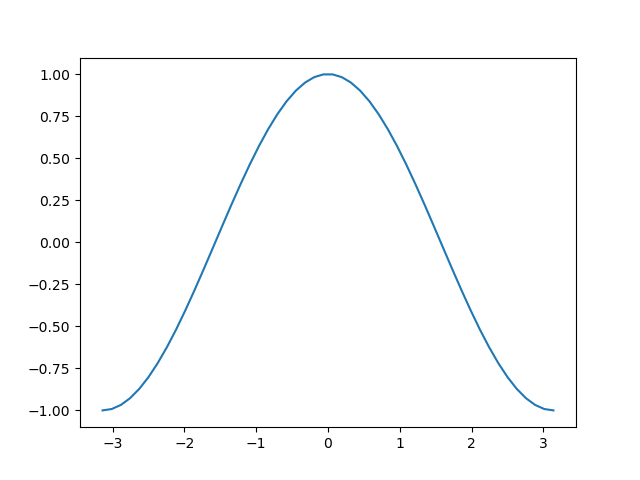
\includegraphics[width=0.7\textwidth]{./data/sen}
  \caption{Esboço do gráfico da função $y=\sen(x)$ no intervalo $[-\pi,\pi]$.}
  \label{fig:sen}
\end{figure}

Gráficos bidimensionais podem ser criados com a função \lstinline+plt.plot(x,y)+, onde \lstinline+x+ e \lstinline+y+ são \lstinline+arrays+ que fornecem os pontos cartesianos $(x_i, y_i)$ a serem plotados. Por exemplo,

\begin{lstlisting}
>>> import matplotlib.pyplot as plt
>>> x = np.linspace(-np.pi, np.pi)
>>> y = np.cos(x)
>>> plt.plot(x,y)
[<matplotlib.lines.Line2D object at 0x7f99f578a370>]
>>> plt.show()
\end{lstlisting}

produz o seguinte esboço do gráfico da função $y=\sen(x)$ no intervalo $[-\pi,\pi]$. Consulte a Figura \ref{fig:sen}.


\begin{obs}
  Matplotlib é uma poderosa ferramenta para a visualização de gráficos. Consulte a galeria de exemplos no seu site oficial
  \begin{center}
    \url{https://matplotlib.org/stable/gallery/index.html}
  \end{center}
\end{obs}

\begin{exr}
  Crie um esboço do gráfico de cada uma das seguintes funções no intervalo indicado:
  \begin{enumerate}[a)]
  \item $y = \cos(x)$, $\left[0, 2\pi\right]$
  \item $y = x^2 - x + 1$, $[-2, 2]$
  \item $y = \tg\left(\frac{\pi}{2}x\right)$, $(-1, 1)$
  \end{enumerate}
\end{exr}

% \bibliography{main}
% \addcontentsline{toc}{section}{Referências Bibliográficas}
%references
% \nocite{Banin, NumPy, PythonTutorial, Ribeiro, TutorialsPoint, SciPy, Wazlawick}

\begin{thebibliography}{99}
  \bibitem{Banin2021a}
    Banin, S.L.. Python 3 - Conceitos e Aplicações - Uma Abordagem Didática, Saraiva: São Paulo, 2021. ISBN: \texttt{978-8536530253}.
    
    \bibitem{NumPy2024a}
    NumpPy Developers. NumPy documentation, versão 1.26, disponível em \url{https://numpy.org/doc/stable/}.

    \bibitem{Ribeiro2021a}
    Ribeiro, J.A.. Introdução à Programação e aos Algoritmos, LTC: São Paulo, 2021. ISBN: \texttt{978-8521636410}.
  
  \bibitem{Matplotlib2024a}
    Hunter, J.; Dale, D.; Firing, E.; Droettboom, M. \& Matplotlib development team. NumPy documentation, versão 3.8.3, disponível em \url{https://matplotlib.org/stable/}.
      
  \bibitem{Python2024a}
    Python Software Foundation. Python documentation, versão 3.12.2, disponível em \url{https://docs.python.org/3/}.
  
  \bibitem{Wazlawick2021a}
    Wazlawick, R.. Introdução a Algoritmos e Programação com Python - Uma Abordagem Dirigida por Testes, Grupo GEN: São Paulo, 2021. ISBN \texttt{978-8595156968}.
  \end{thebibliography}
  

\end{document}
